\section{Vorbereitung}
\subsection{Dispersionsgebiet und Auflösungsvermögen}
Zur Auswertung des Versuchs ist es zunächst noch notwendig das Auflösungsvermögen und das Dispersionsgebiet für die zu untersuchenden Spektralinien zu bestimmen. Mit (\ref{eq:auf}) und
(\ref{eq:disp}) ergibt sich:
\begin{table}[]
\centering
\begin{tabular}{c|cc}
 & Rot  & Blau\\
 \hline
$A$ & 209064  & 285458 \\
$\updelta \lambda_\text{D}$ & $48{,}94\,\si{\pico\meter}$ &$27{,}94\,\si{\pico\meter}$
\end{tabular}
\end{table}
Hierbei sind die Parameter der Lummer-Gehrke-Platte
\begin{align}
&d=4\,\si{\nm}\nonumber\\
&L=120\,\si{\mm}\nonumber\\
&n\left(@644\,\si{\nm}\right)=1{,}4567\nonumber\\
&n\left(@480\,\si{\nm}\right)=1{,}4635\nonumber
\end{align}
\subsection{Optische Übergänge in Cadmium-Atomen}
Die Termschemata der blauen und roten Linie sind in den Abbildungen \ref{fig:blue} und \ref{fig:red} dargestellt. Für die blaue Linie bestimmen sich die Landé-Faktoren der Energieniveaus gemäß (\ref{eq:lande}) zu:
\begin{table}[H]
\centering
\begin{tabular}{c|c}
 & $g_J$\\
 \hline
$^3P_1$  & 1{,}5 \\
$^3S_1$&2
\end{tabular}
\end{table}
Für die rote Linie liegt der normale Zeeman-Effekt vor weswegen $g_J=1$ gilt. Die daraus folgenden Energiedifferenzen der Niveaus $\upDelta E$ sind in Tabelle \ref{tab:ediff} dargestellt.
\begin{table}[]
\centering
\begin{tabular}{c|ccc}
 &$\upDelta m = 1$&$\upDelta m=0$&$\upDelta m = -1$ \\
 \hline
Rot&$-\upmu_BB$&$0$&$\upmu_BB$\\
Blau $(m_1=+1)$&$-$&$-\frac{1}{2}\upmu_BB$&$\frac{3}{2}\upmu_BB$\\
Blau $(m_1=0)$&$-2\upmu_BB$&$0$&$2\upmu_BB$\\
Blau $(m_1=-1)$&$-\frac{3}{2}\upmu_BB$&$\frac{1}{2}\upmu_BB$&-
\end{tabular}
\label{tab:ediff}
\end{table}
\begin{figure}
  \centering
  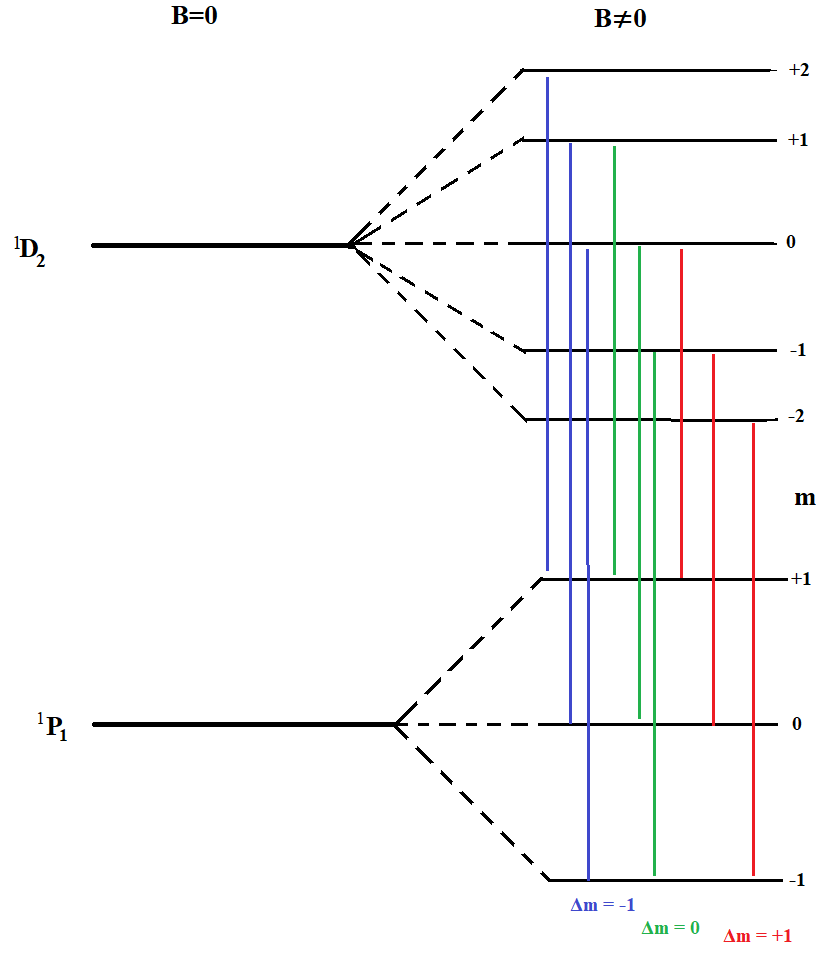
\includegraphics[scale=0.4]{Bilder/1Termschema.png}
  \caption{Schematisches Termschema der Zeeman-Aufspaltung bei der roten Linie.}
\end{figure}
\begin{figure}
  \centering
  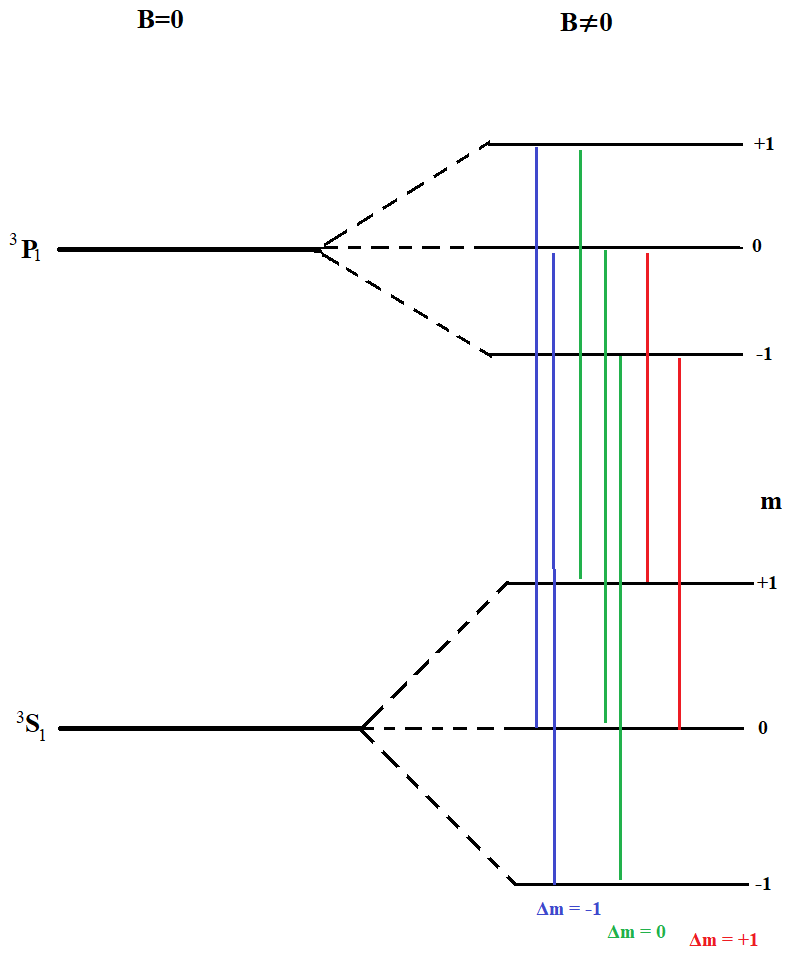
\includegraphics[scale=0.4]{Bilder/2Termschema.png}
  \caption{Schematisches Termschema der Zeeman-Aufspaltung bei der roten Linie.}
\end{figure}

\subsection{Optimale Magnetfeldstärke}
Um garantieren zu können, dass die Aufspaltungen innerhalb des Dispersionsgebiets liegen ist es notwendig die optimale Magnetfeldstärke zu bestimmen. Mit den vorhandenen Gleichungen lässt sich zeigen, dass zwischen B-Feld und Dispersionsgebiet gilt:
\begin{equation}
B=\frac{hc}{4\lambda^2}\upDelta\lambda_\text{D}\frac{1}{g\upmu_B}\,.
\end{equation}
Mit den bereits berechneten Dispersionsgebieten folgt
\begin{align}
B\left(\lambda=480\,\si{\nm}, g=1{,}75\right)&=371{,}20\,\si{\milli\tesla}\nonumber\\
B\left(\lambda=480\,\si{\nm}, g=0{,}5\right)&=1299{,}21\,\si{\milli\tesla}\nonumber\\
B\left(\lambda=643{,}8\,\si{\nm}, g=1\right)&=632{,}28\,\si{\milli\tesla}\nonumber
\end{align}
